\documentclass{ctexart}

\usepackage{amsmath}
\usepackage{tikz}
\usetikzlibrary{arrows.meta}

\definecolor{boundarycolor}{cmyk}{1,0,0,0}%Cyan
\definecolor{thirdcolor}{cmyk}{0.82,0.00,0.04,0.30}%LightSeaGreen
\definecolor{fillcolor}{cmyk}{0.12,0,0,0}%LightCyan

\begin{document}	
	
	\begin{figure}
		
		\centering
		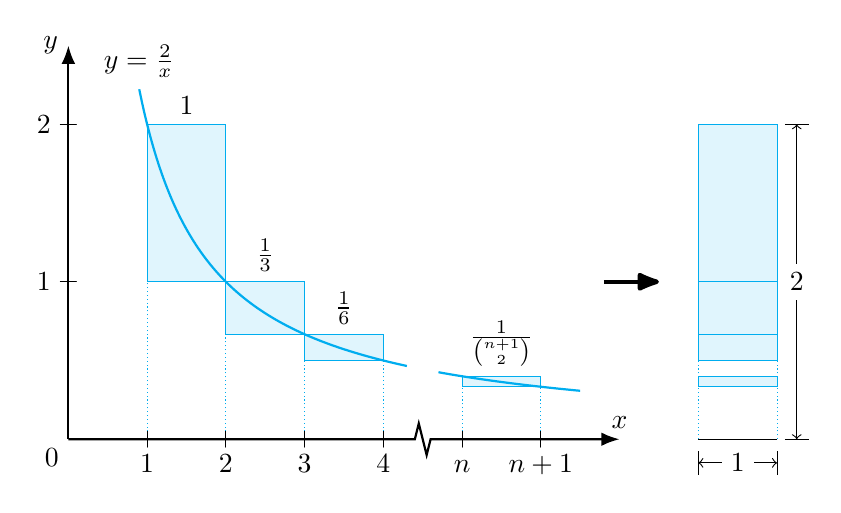
\begin{tikzpicture}
			%曲线上的矩形
			\filldraw[draw=boundarycolor,fill=fillcolor](1,4)rectangle(2,2);
			\filldraw[draw=boundarycolor,fill=fillcolor](2,2)rectangle(3,4/3);
			\filldraw[draw=boundarycolor,fill=fillcolor](3,4/3)rectangle(4,1);
			\filldraw[draw=boundarycolor,fill=fillcolor](5,4/5)rectangle(6,2/3);
			%矩形面积
			\node at (1.5,4)[above]{$1$};
			\node at (2.5,2)[above]{$\frac{1}{3}$};
			\node at (3.5,4/3)[above]{$\frac{1}{6}$};
			\node at (5.5,4/5)[above]{$\frac{1}{\binom{n+1}{2}}$};
			%虚线
			\draw[densely dotted,boundarycolor](1,0)--(1,4);
			\draw[densely dotted,boundarycolor](2,0)--(2,2);
			\draw[densely dotted,boundarycolor](3,0)--(3,4/3);
			\draw[densely dotted,boundarycolor](4,0)--(4,1);
			\draw[densely dotted,boundarycolor](6,0)--(6,2/3);
			\draw[densely dotted,boundarycolor](5,0)--(5,4/5);
			%曲线
			\node at (0.9,4.8){$y=\frac{2}{x}$};
			\draw [domain=0.9:4.3,samples=100,smooth,variable=\t,color=boundarycolor,thick] plot({\t},{4/(\t)});
			\draw [domain=4.7:6.5,samples=100,smooth,variable=\t,color=boundarycolor,thick] plot({\t},{4/(\t)});
			%坐标轴
			\draw[-{Latex},thick] (0,0)--(4.4,0)--(4.45,0.2)--(4.55,-0.2)--(4.6,0)--(7,0) node[above] {$x$};
			\draw[-{Latex},thick] (0,0)--(0,5) node[left] {$y$};
			\draw[thin,line join=round,line cap=round](1,-0.1)--(1,0.1)node[below=5pt]{$1$};
			\draw[thin,line join=round,line cap=round](2,-0.1)--(2,0.1)node[below=5pt]{$2$};
			\draw[thin,line join=round,line cap=round](3,-0.1)--(3,0.1)node[below=5pt]{$3$};
			\draw[thin,line join=round,line cap=round](4,-0.1)--(4,0.1)node[below=5pt]{$4$};
			\draw[thin,line join=round,line cap=round](5,-0.1)--(5,0.1)node[below=7pt]{$n$};
			\draw[thin,line join=round,line cap=round](6,-0.1)--(6,0.1)node[below=5pt]{$n+1$};
			\draw[thin,line join=round,line cap=round](-0.1,2)node[left]{$1$}--(0.1,2);
			\draw[thin,line join=round,line cap=round](-0.1,4)node[left]{$2$}--(0.1,4);
			\node at (0,0)[below left]{$0$};
			
			%中间箭头
			\draw[-{Latex[round]},ultra thick](6.8,2)--(7.5,2);
			
			%矩形堆积
			\filldraw[draw=boundarycolor,fill=fillcolor](8,4)rectangle(9,2);
			\filldraw[draw=boundarycolor,fill=fillcolor](8,2)rectangle(9,4/3);
			\filldraw[draw=boundarycolor,fill=fillcolor](8,4/3)rectangle(9,1);
			\filldraw[draw=boundarycolor,fill=fillcolor](8,4/5)rectangle(9,2/3);
			\draw[densely dotted,boundarycolor](8,0)--(8,4);
			\draw[densely dotted,boundarycolor](9,0)--(9,4);
			\draw(8,0)--(9,0);
			%长和宽
			\draw[{Classical TikZ Rightarrow}-{Classical TikZ Rightarrow}](8,-0.3)--(9,-0.3);
			\node [fill=white] at (8.5,-0.3) [minimum size=5pt] {$1$};
			\draw(8,-0.45)--(8,-0.15);
			\draw(9,-0.45)--(9,-0.15);
			\draw[{Classical TikZ Rightarrow}-{Classical TikZ Rightarrow}](9.25,0)--(9.25,4);
			\node [fill=white] at (9.25,2) [minimum size=5pt] {$2$};
			\draw(9.1,0)--(9.4,0);
			\draw(9.1,4)--(9.4,4);
		\end{tikzpicture}
		\caption{三角形数倒数和的无字证明}
	\end{figure}
	
\end{document}